\section{Introduction}

Many corporations process a lot of interesting data in the form of Business Timeseries. These can be customer related such as purchases, interactions through consultations, support, incident reports, usage of the service and so forth. They can also be about internal processes that cannot be attributed to a single customer, such as infrastructures providing services to multiple customers. These timeseries can provide insights on how an aspect of a company performed in the past, but they also provide the foundation to create forecasts. 

The predictions that an organization wants to make could be a single step into the future, useful for operation automation, i.e., scaling services, anomaly detection, alerting, etc. Or it is desired to create forecasts long into the future to anticipate growth, scale the business, make strategic decisions, or optimize logistics or processes.

\subsection{Types of Timeseries}

Timeseries are typically uni-variate, where we have one value per point in time. We use those values to extract the underlying patterns to be able to forecast the future horizon of that timeseries. E.g., we can collect metrics of a river's temperature every 15 minutes over the period of years. We will likely find daily and yearly seasonalities in this timeseries as the river temperature is influenced by day light and the air temperature. Thus, the temperature is colder at night and in winter.

With multi-variate timeseries we have multiple values per point in time. E.g., we can collect air temperature, level of cloudiness, air humidity, air pressure, etc. and we try to predict the river's temperature with those metrics. This is traditionally done with regression type models.

The last case is that we start with a uni-variate temperature, say the river's temperature, and we add exogenous timeseries, like the air temperature. A good model will learn the dependency between the regressor variables and the variable to be predicted. The problem now is that we need the air temperature data for the future to be available when we try to predict the river's temperature. This is not always possible. An example where it is possible is when we try to predict sales of products and we have a calendar when advertisements of the products will go online. A model could learn how the advertisement variable impacts the sales timeseries and add its effect to the forecast.

Timeseries are generally generated by collecting metrics of an underlying event stream. E.g., a timeseries on the amount of sales of a product uses each sell event as the underlying data stream. The sell events are then aggregated or binned into equally apart time slots which we will call frequency or resolution. If we choose a high frequency, e.g., 5 seconds, we will likely end up having many zeros and occasionally a one in our timeseries. In most cases this timeseries should be further aggregated into larger bins. The resolution of a timeseries needs to be chosen with its use case in mind. It is of course a good idea to record data in a very high resolution, so we have the possibility to aggregate the series further in any resolution we need later. Down sampling of timeseries is also possible, where the data points are linearly spread over smaller time slots. However, a down sampled timeseries should not be used to create forecasts because it contains inaccurate information of the distribution of metrics.


\subsection{Timeseries Forecasting Models}

Timeseries forecasting is a field that does not share many learning methods with other traditional machine learning fields like computer vision, natural language processing, speech recognition, etc. Methods like deep learning have been applied, but were not as successful, and at the same time more costly to train, than methods coming from the field. It is also hard to beat baseline methods like Na\"ive and Seasonal Na\"ive, where the model takes the last value and predicts that this is the future value. And with Seasonal Na\"ive, the last value of the same period is looked at. There are slight variations of this by taking the last, mean, median or drift, but they remain very easy to understand and are similar to what a human would do when asked to forecast a uni-variate timeseries.

One possibility to model a timeseries is with three separate components that we additively or multiplicatively combine to a prediction model. We add the trend or growth \(g(t)\) modeling nonperiodic changes, the seasonality \(s(t)\) modeling the periodic changes, the holidays and events \(h(t)\) modeling single data point effects which are potentially irregular, and the error term \(\epsilon_t\) that is assumed to be normally distributed.

\begin{equation}
    y(t)=g(t)+s(t)+h(t)+\epsilon_t
    \label{eq:fullTrendModel}
\end{equation}

This type of model is an additive linear model for example used by Linear Regression type models and Prophet \cite{prophet}. Through the nature of this component model, we can decompose timeseries as shown in figure \ref{fig:stl-decomposition}.


\begin{figure*}
\centerline{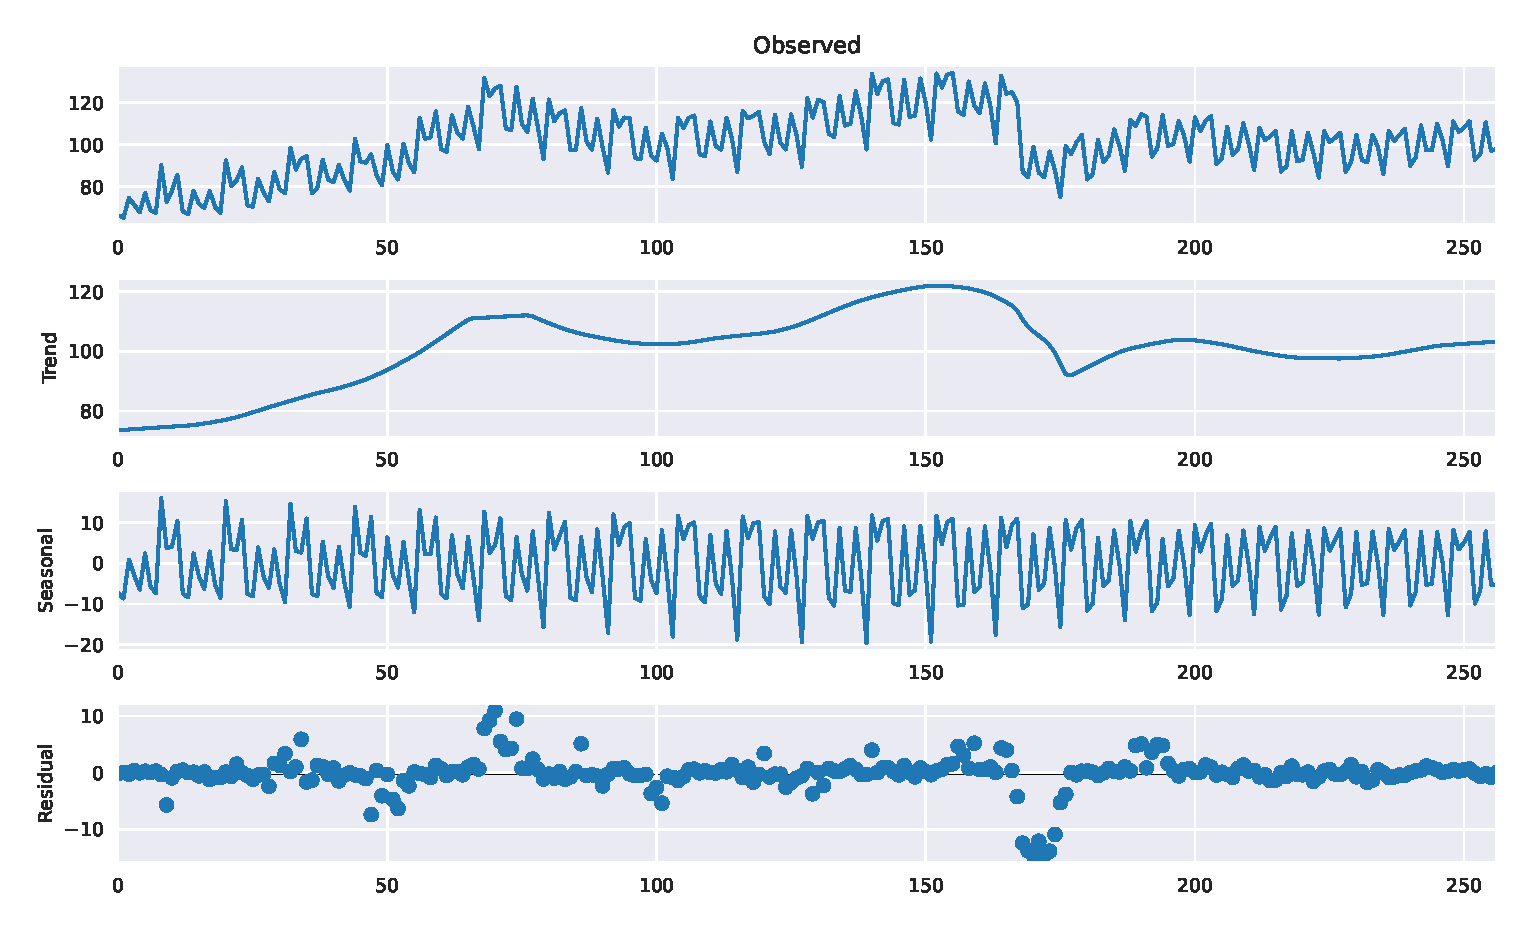
\includegraphics[scale=.6]{Figures/stl.eps}}
\caption{An example timeseries decomposed into trend, seasonal and residual components by STL \cite{STL} (Seasonal and Trend decomposition using Loess). STL works iteratively by removing a trend estimate, then smoothing the cyclic sub series to get the seasonal component. The seasonality is smoothed again, and we go back to get a more accurate trend estimate. This gets repeated several times to improve the accuracy. Such decompositions are also possible when using another model such as Prophet which uses Fourier series.}
\label{fig:stl-decomposition}
\end{figure*}

Fitting a more complex model to a timeseries does only result in a significant improvement if the chosen model makes sense for that use case and correct hyper-parameters have been specified. There are more complex models such as ARIMA \cite{ARIMA} (Auto-Regressive Integrated Moving Average) that tries to model the autocorrelations of the timeseries. Holt Winter's method \cite{HOLT} uses weighted averages of past observations, with the weights decaying exponentially as the observations get older. 
Those types of models do not include too many hyper-parameters yet specifying them correctly is not easy and only experienced analysts are capable of doing that.

Thus, it becomes time intensive and tricky to find the best model and parameters. If enough computing capacity is available and only a few timeseries shall be forecasted, we can fit a zoo of models to the timeseries and elect the best performing model. The size of a mostly complete model zoo for timeseries problems would typically be 15 - 30. But then come the hyper-parameters of each model. To truly select the best model and parameters, we need to compare all model and hyper-parameter combinations with each other in the same ranking. This grid search is expensive as the models to be fitted easily grow to thousands or tens of thousands. If fitting one model takes one second, and we are assuming we are doing this in series, we would wait hours to find the best model of a single timeseries. But we maybe have hundreds of thousands timeseries. This quickly leads to a waiting time of many years, which is not feasible. 

Another option is to select a single capable method, which performs reasonably on most timeseries and call this the model to rule them all. This approach has been taken by many companies. The model often chosen is Prophet \cite{prophet}. It can fit trends with a limiting capacity, do automatic changepoint detection, extract multiple seasonalities using Fourier series, and incorporate holiday effects into a prediction. This makes it an ideal candidate to apply to almost every timeseries forecasting problem. Using a single model has its drawbacks as well. For one, there might be timeseries in a dataset that are static, meaning they only ever contain a static value that never changes, or they follow a perfect single seasonality period. Fitting Prophet to these timeseries will likely result in a higher error term and cost more compute power than a Na\"ive method.

Timeseries forecasting is an active field of research and there are several competitions held every year to encourage people finding the best methods. The winning methods usually revolve around gradient boosted machines (GBM) with auto-regressors \cite{gbm}. These types of models are great at forecasting, but they are also inherently slow. Therefore several new optimized GBM libraries have sprouted up like LightGBM \cite{lightgbm} and XGBoost \cite{xgboost}. To win a competition, one needs to achieve the highest score, and compute cost does not matter. However, in a real-world scenario, compute cost does matter. Explainability of a model can also matter if these forecasts must be consumed by humans to make decisions upon.

Ideally, we would like to have a system that can suggest the best model automatically given the forecasting scenario, the data and the requirements in form of time, explainability and accuracy.

\subsection{Datasets}

Finding timeseries datasets initially seems trivial. When following tutorials for timeseries forecasting, the libraries usually provide an integrated or readily downloadable dataset to play around with. These toy datasets usually have been selected to highlight the strengths of a library and its default parameters, making forecasting seem easy. Real-world datasets contain a lot more error terms and hidden patterns if any. Finding a wide range of datasets with enough variation to satisfy specific needs might become a hard task.

Competition datasets usually provide a good challenge to a timeseries forecaster. Yet, those timeseries are usually made to support one forecasting task in mind, thus they do not provide a heterogeneous dataset. If one tries to fit several models to all the timeseries within such a dataset, they will probably find a wide range of winning models and a clear overall winner. However, trying to figure out which model should be selected per timeseries before trying them all out, is a hard problem, as they all have similar characteristics.


\subsection{Timeseries Prediction Tasks}

We will distinguish between different timeseries prediction tasks that will lead to different models excelling at them.

The first forecasting task is to predict the short-term future. This can be a single step into the future or several but few. E.g if we have a dataset with one data point per day, we could predict the value for the next day. Similarly, if we have a dataset with a 5 minute resolution, we could predict the data point for the following 5 minutes. In this task we tend to have less long-term dependencies and focus more on the short-term dependencies of the timeseries. The long-term trend is also not as relevant here. The error metric on the forecast will also show little differences if we use different models, as we are only predicting one point.

A harder task is to forecast the long-term future. Here we need to take trend and seasonality into account. The error metric can also easily grow as we accumulate errors over multiple data points.

Another interesting task is to find anomalies in timeseries data. One can analyze a recorded timeseries and find anomalies in the past data. There are simple methods like taking the \(n^{th}\) percentile and comparing each datapoint to check if it lies within it, otherwise mark it as an anomaly. There are also methods that use local regression (e.g., LOESS) to fit a smoothed curve and check if there are points that are outside the sensitivity bounds. We will not focus on anomaly detection in past data in this work. We produce anomalies if the incoming data is outside of forecasting bounds instead.

Anomaly Detection is also relevant in systems that produce new timeseries data points live that need to be classified as being an anomaly or not. This is typically used in operations scenarios, where a human or an automated system needs to act if there are anomalies found, as it indicates that the underlying behavior of the data has changed. This task can also be solved by methods of finding anomalies in past data, by adding the incoming data to the existing timeseries and run one of the methods over it. The other option is to forecast the timeseries a few steps into the future with a prediction bound and compare incoming data against it. If the incoming data is out of bounds, we mark the data point as anomaly. This is the anomaly detection approach what we will focus on in this work.
